\documentclass[tikz, letterpaper,12pt]{article}

\usepackage{geometry}
\usepackage{pslatex}
\usepackage{fancyhdr}
\usepackage{graphicx}
\usepackage{color}
\usepackage{subcaption}
\usepackage{float}
\usepackage{tikz}
\usepackage{setspace}
\geometry{ margin = 1.0in }

\usetikzlibrary{matrix,backgrounds}
\usepackage{listings}
\usepackage{color}

\usepackage[fleqn]{mathtools}
\DeclarePairedDelimiter\ceil{\lceil}{\rceil}
\DeclarePairedDelimiter\floor{\lfloor}{\rfloor}

\definecolor{dkgreen}{rgb}{0,0.6,0}
\definecolor{gray}{rgb}{0.5,0.5,0.5}
\definecolor{mauve}{rgb}{0.58,0,0.82}

\lstset{frame=tb,
  language=Java,
  aboveskip=3mm,
  belowskip=1mm,
  showstringspaces=false,
  columns=flexible,
  basicstyle={\small\ttfamily},
  numbers=none,
  numberstyle=\tiny\color{gray},
  keywordstyle=\color{blue},
  commentstyle=\color{dkgreen},
  stringstyle=\color{mauve},
  breaklines=true,
  breakatwhitespace=true,
  tabsize=3
}

\usepackage{amssymb, amsthm, bm, nicefrac}

\newcommand{\xto}[1]{\xrightarrow{#1}}
\newcommand{\NN}{\mathbb{N}}
\newcommand{\ZZ}{\mathbb{Z}}
\newcommand{\QQ}{\mathbb{Q}}
\newcommand{\RR}{\mathbb{R}}
\newcommand{\CC}{\mathbb{C}}
\newcommand{\abs}[1]{\left|#1\right|}
\newcommand{\norm}[1]{\left\|#1\right\|}
\newcommand{\normal}{\trianglelefteq}
\renewcommand{\qedsymbol}{\rule{0.7em}{0.7em}}

\newcommand{\aaa}[1]{\hspace{0.65cm}\parbox[t]{15.3cm}{#1}}
\newcommand{\aab}[1]{\hspace{1.15cm}\parbox[t]{15.0cm}{#1}}
\newcommand{\aac}[1]{\hspace{1.65cm}\parbox[t]{15.0cm}{#1}}
\newcommand{\aad}[1]{\hspace{2.15cm}\parbox[t]{15.0cm}{#1}}
\newcommand{\aae}[1]{\hspace{2.65cm}\parbox[t]{15.0cm}{#1}}
\newcommand{\aaf}[1]{\hspace{3.15cm}\parbox[t]{15.0cm}{#1}}
\newcommand{\aag}[1]{\hspace{3.65cm}\parbox[t]{15.0cm}{#1}}
\newcommand{\aaA}[2]{\hspace{0.5cm} {\tikz[overlay] \draw (0.1, -0.1) -- (0.1, #1 * -1.5em + 0.6em);} \parbox[t]{15.0cm}{#2}}
\newcommand{\aaB}[2]{\hspace{1.0cm} {\tikz[overlay] \draw (0.1, -0.1) -- (0.1, #1 * -1.5em + 0.6em);} \parbox[t]{15.0cm}{#2}}
\newcommand{\aaC}[2]{\hspace{1.5cm} {\tikz[overlay] \draw (0.1, -0.1) -- (0.1, #1 * -1.5em + 0.6em);} \parbox[t]{15.0cm}{#2}}
\newcommand{\aaD}[2]{\hspace{2.0cm} {\tikz[overlay] \draw (0.1, -0.1) -- (0.1, #1 * -1.5em + 0.6em);} \parbox[t]{15.0cm}{#2}}
\newcommand{\aaE}[2]{\hspace{2.5cm} {\tikz[overlay] \draw (0.1, -0.1) -- (0.1, #1 * -1.5em + 0.6em);} \parbox[t]{15.0cm}{#2}}
\newcommand{\aaF}[2]{\hspace{3.0cm} {\tikz[overlay] \draw (0.1, -0.1) -- (0.1, #1 * -1.5em + 0.6em);} \parbox[t]{15.0cm}{#2}}
\newcommand{\aaG}[2]{\hspace{3.5cm} {\tikz[overlay] \draw (0.1, -0.1) -- (0.1, #1 * -1.5em + 0.6em);} \parbox[t]{15.0cm}{#2}}
\newcommand{\xxx}{\par\vspace{0.1cm}}

%%% TODO modify these variables %%%
\def\homeworknum{3}
\def\namex{Param Somane}
\def\accessx{pss5256}
%%%%

\pagestyle{fancy}
\lhead{{\bf CMPSC 465 Fall 2020}}
\chead{{\bf Writing Assignment~\homeworknum}}
\rhead{{\bf October 16, 2020}}

\newcounter{problemid}\stepcounter{problemid}
\def\newproblem{\vspace*{0.01cm}{\bf Problem~\arabic{problemid}\stepcounter{problemid}}\hfill\fbox{\parbox{0.16\textwidth}{\bf Points:}}\par}

\setlength\parindent{0em}
\setlength\parskip{8pt}
\setlength{\fboxsep}{6pt}
\newtheorem{definition}{Definition}
\newtheorem{property}{Property}
\newtheorem{claim}{Claim}
\newtheorem{fact}{Fact}
\newtheorem{corollary}{Corollary}
\newtheorem{lemma}{Lemma}

\makeatletter
\newenvironment{proof*}[1][\proofname]{\par
  \pushQED{\qed}%
  \normalfont \partopsep=\z@skip \topsep=\z@skip
  \trivlist
  \item[\hskip\labelsep
        \itshape
    #1\@addpunct{.}]\ignorespaces
}{%
  \popQED\endtrivlist\@endpefalse
}
\makeatother

\begin{document}

\framebox[\textwidth]{
	\parbox{0.96\textwidth}{
		\parbox{0.08\textwidth}{\bf Name:}\parbox{0.65\textwidth}{\namex}\parbox{0.12\textwidth}{\bf Access ID:}\parbox{0.14\textwidth}{\accessx}
	}
}

%% your solutions %%%
\newproblem
1. We run Dijkstra's algorithm on the given graph. We denote NULL by $\phi$. We utilize three data structures for this algorithm, namely the priority queue $PQ$, $dist[]$ array, $prev[]$ array, and {$S:=\{v\in V\mid  distance(s, v)$ has been found$\}$}. 

\qquad\qquad\qquad$dist$\qquad\quad\qquad\qquad\qquad\qquad\qquad$prev$\qquad\qquad\qquad\qquad\qquad$PQ\;\;minimum$

\textit{Initialization}\newline
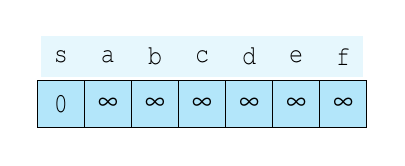
\begin{tikzpicture}[font=\ttfamily,
array/.style={matrix of nodes,nodes={draw, minimum size=7mm, minimum
    width=1.7em,minimum height=1.7em, anchor=center, fill=cyan!30},column sep=-\pgflinewidth, row sep=0.5mm, nodes in empty cells,
row 1/.style={nodes={draw=none, fill=none, minimum size=5mm}}}]
\matrix[array] (array) {
s & a & b & c & d & e & f\\
0  & $\infty$ & $\infty$ & $\infty$ & $\infty$ & $\infty$ & $\infty$\\};
\begin{scope}[on background layer]
\fill[cyan!10] (array-1-1.north west) rectangle (array-1-7.south east);
\end{scope}
\end{tikzpicture}
\qquad
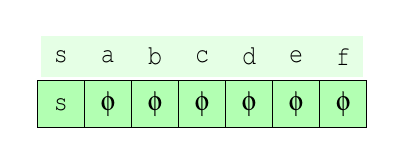
\begin{tikzpicture}[font=\ttfamily,
array/.style={matrix of nodes,nodes={draw, minimum size=7mm, minimum
    width=1.7em,minimum height=1.7em, anchor=center, fill=green!30},column sep=-\pgflinewidth, row sep=0.5mm, nodes in empty cells,
row 1/.style={nodes={draw=none, fill=none, minimum size=5mm}}}]
\matrix[array] (array) {
s & a & b & c & d & e & f\\
s  & $\phi$ & $\phi$ & $\phi$ & $\phi$ & $\phi$ & $\phi$\\};
\begin{scope}[on background layer]
\fill[green!10] (array-1-1.north west) rectangle (array-1-7.south east);
\end{scope}
\end{tikzpicture}
\raisebox{1.3em}{
\begin{tikzpicture}[font=\ttfamily]
\qquad $\;\;\;\;\;s\;\;-\;\;$\quad $distance(s,s)=0$
\end{tikzpicture}}

\textit{Iteration 1}\newline
Delete s from $PQ$ and $S=\{s\}$\newline
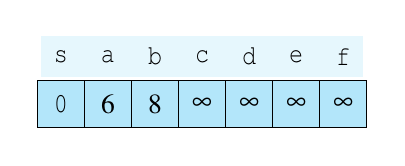
\begin{tikzpicture}[font=\ttfamily,
array/.style={matrix of nodes,nodes={draw, minimum size=7mm, minimum
    width=1.7em,minimum height=1.7em, anchor=center, fill=cyan!30},column sep=-\pgflinewidth, row sep=0.5mm, nodes in empty cells,
row 1/.style={nodes={draw=none, fill=none, minimum size=5mm}}}]
\matrix[array] (array) {
s & a & b & c & d & e & f\\
0  & $6$ & $8$ & $\infty$ & $\infty$ & $\infty$ & $\infty$\\};
\begin{scope}[on background layer]
\fill[cyan!10] (array-1-1.north west) rectangle (array-1-7.south east);
\end{scope}
\end{tikzpicture}
\qquad
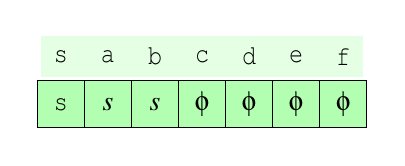
\begin{tikzpicture}[font=\ttfamily,
array/.style={matrix of nodes,nodes={draw, minimum size=7mm, minimum
    width=1.7em,minimum height=1.7em, anchor=center, fill=green!30},column sep=-\pgflinewidth, row sep=0.5mm, nodes in empty cells,
row 1/.style={nodes={draw=none, fill=none, minimum size=5mm}}}]
\matrix[array] (array) {
s & a & b & c & d & e & f\\
s  & $s$ & $s$ & $\phi$ & $\phi$ & $\phi$ & $\phi$\\};
\begin{scope}[on background layer]
\fill[green!10] (array-1-1.north west) rectangle (array-1-7.south east);
\end{scope}
\end{tikzpicture}
\raisebox{1.3em}{
\begin{tikzpicture}[font=\ttfamily]
\qquad $\;\;\;\;\;a\;\;-\;\;$\quad $distance(s,a)=6$
\end{tikzpicture}}

\textit{Iteration 2}\newline
Delete a from $PQ$ and $S=\{s,a\}$\newline
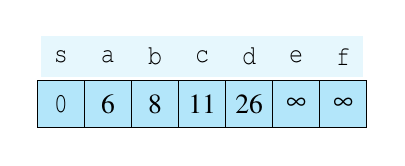
\begin{tikzpicture}[font=\ttfamily,
array/.style={matrix of nodes,nodes={draw, minimum size=7mm, minimum
    width=1.7em,minimum height=1.7em, anchor=center, fill=cyan!30},column sep=-\pgflinewidth, row sep=0.5mm, nodes in empty cells,
row 1/.style={nodes={draw=none, fill=none, minimum size=5mm}}}]
\matrix[array] (array) {
s & a & b & c & d & e & f\\
0  & $6$ & $8$ & $11$ & $26$ & $\infty$ & $\infty$\\};
\begin{scope}[on background layer]
\fill[cyan!10] (array-1-1.north west) rectangle (array-1-7.south east);
\end{scope}
\end{tikzpicture}
\qquad
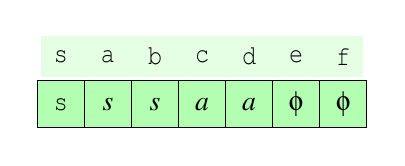
\begin{tikzpicture}[font=\ttfamily,
array/.style={matrix of nodes,nodes={draw, minimum size=7mm, minimum
    width=1.7em,minimum height=1.7em, anchor=center, fill=green!30},column sep=-\pgflinewidth, row sep=0.5mm, nodes in empty cells,
row 1/.style={nodes={draw=none, fill=none, minimum size=5mm}}}]
\matrix[array] (array) {
s & a & b & c & d & e & f\\
s  & $s$ & $s$ & $a$ & $a$ & $\phi$ & $\phi$\\};
\begin{scope}[on background layer]
\fill[green!10] (array-1-1.north west) rectangle (array-1-7.south east);
\end{scope}
\end{tikzpicture}
\raisebox{1.3em}{
\begin{tikzpicture}[font=\ttfamily]
\qquad $\;\;\;\;\;b\;\;-\;\;$\quad $distance(s,b)=8$
\end{tikzpicture}}

\textit{Iteration 3}\newline
Delete b from $PQ$ and $S=\{s,a,b\}$\newline
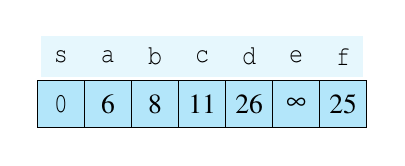
\begin{tikzpicture}[font=\ttfamily,
array/.style={matrix of nodes,nodes={draw, minimum size=7mm, minimum
    width=1.7em,minimum height=1.7em, anchor=center, fill=cyan!30},column sep=-\pgflinewidth, row sep=0.5mm, nodes in empty cells,
row 1/.style={nodes={draw=none, fill=none, minimum size=5mm}}}]
\matrix[array] (array) {
s & a & b & c & d & e & f\\
0  & $6$ & $8$ & $11$ & $26$ & $\infty$ & $25$\\};
\begin{scope}[on background layer]
\fill[cyan!10] (array-1-1.north west) rectangle (array-1-7.south east);
\end{scope}
\end{tikzpicture}
\qquad
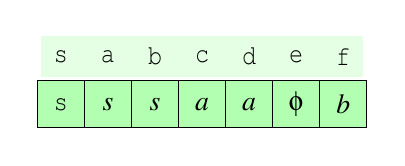
\begin{tikzpicture}[font=\ttfamily,
array/.style={matrix of nodes,nodes={draw, minimum size=7mm, minimum
    width=1.7em,minimum height=1.7em, anchor=center, fill=green!30},column sep=-\pgflinewidth, row sep=0.5mm, nodes in empty cells,
row 1/.style={nodes={draw=none, fill=none, minimum size=5mm}}}]
\matrix[array] (array) {
s & a & b & c & d & e & f\\
s  & $s$ & $s$ & $a$ & $a$ & $\phi$ & $b$\\};
\begin{scope}[on background layer]
\fill[green!10] (array-1-1.north west) rectangle (array-1-7.south east);
\end{scope}
\end{tikzpicture}
\raisebox{1.3em}{
\begin{tikzpicture}[font=\ttfamily]
\qquad $\;\;\;\;\;c\;\;-\;\;$\quad $distance(s,c)=11$
\end{tikzpicture}}

\textit{Iteration 4}\newline
Delete c from $PQ$ and $S=\{s,a,b,c\}$\newline
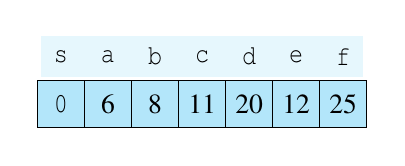
\begin{tikzpicture}[font=\ttfamily,
array/.style={matrix of nodes,nodes={draw, minimum size=7mm, minimum
    width=1.7em,minimum height=1.7em, anchor=center, fill=cyan!30},column sep=-\pgflinewidth, row sep=0.5mm, nodes in empty cells,
row 1/.style={nodes={draw=none, fill=none, minimum size=5mm}}}]
\matrix[array] (array) {
s & a & b & c & d & e & f\\
0  & $6$ & $8$ & $11$ & $20$ & $12$ & $25$\\};
\begin{scope}[on background layer]
\fill[cyan!10] (array-1-1.north west) rectangle (array-1-7.south east);
\end{scope}
\end{tikzpicture}
\qquad
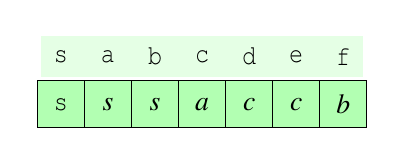
\begin{tikzpicture}[font=\ttfamily,
array/.style={matrix of nodes,nodes={draw, minimum size=7mm, minimum
    width=1.7em,minimum height=1.7em, anchor=center, fill=green!30},column sep=-\pgflinewidth, row sep=0.5mm, nodes in empty cells,
row 1/.style={nodes={draw=none, fill=none, minimum size=5mm}}}]
\matrix[array] (array) {
s & a & b & c & d & e & f\\
s  & $s$ & $s$ & $a$ & $c$ & $c$ & $b$\\};
\begin{scope}[on background layer]
\fill[green!10] (array-1-1.north west) rectangle (array-1-7.south east);
\end{scope}
\end{tikzpicture}
\raisebox{1.3em}{
\begin{tikzpicture}[font=\ttfamily]
\qquad $\;\;\;\;\;e\;\;-\;\;$\quad $distance(s,e)=12$
\end{tikzpicture}}

\textit{Iteration 5}\newline
Delete e from $PQ$ and $S=\{s,a,b,c,e\}$\newline
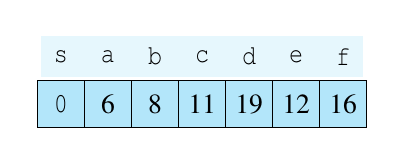
\begin{tikzpicture}[font=\ttfamily,
array/.style={matrix of nodes,nodes={draw, minimum size=7mm, minimum
    width=1.7em,minimum height=1.7em, anchor=center, fill=cyan!30},column sep=-\pgflinewidth, row sep=0.5mm, nodes in empty cells,
row 1/.style={nodes={draw=none, fill=none, minimum size=5mm}}}]
\matrix[array] (array) {
s & a & b & c & d & e & f\\
0  & $6$ & $8$ & $11$ & $19$ & $12$ & $16$\\};
\begin{scope}[on background layer]
\fill[cyan!10] (array-1-1.north west) rectangle (array-1-7.south east);
\end{scope}
\end{tikzpicture}
\qquad
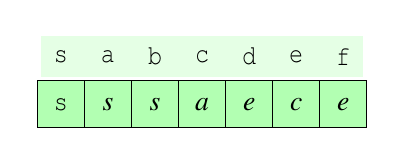
\begin{tikzpicture}[font=\ttfamily,
array/.style={matrix of nodes,nodes={draw, minimum size=7mm, minimum
    width=1.7em,minimum height=1.7em, anchor=center, fill=green!30},column sep=-\pgflinewidth, row sep=0.5mm, nodes in empty cells,
row 1/.style={nodes={draw=none, fill=none, minimum size=5mm}}}]
\matrix[array] (array) {
s & a & b & c & d & e & f\\
s  & $s$ & $s$ & $a$ & $e$ & $c$ & $e$\\};
\begin{scope}[on background layer]
\fill[green!10] (array-1-1.north west) rectangle (array-1-7.south east);
\end{scope}
\end{tikzpicture}
\raisebox{1.3em}{
\begin{tikzpicture}[font=\ttfamily]
\qquad $\;\;\;\;\;f\;\;-\;\;$\quad $distance(s,f)=16$
\end{tikzpicture}}
\newpage
\textit{Iteration 6}\newline
Delete f from $PQ$ and $S=\{s,a,b,c,e,f\}$\newline
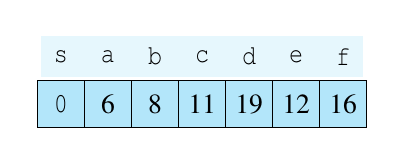
\begin{tikzpicture}[font=\ttfamily,
array/.style={matrix of nodes,nodes={draw, minimum size=7mm, minimum
    width=1.7em,minimum height=1.7em, anchor=center, fill=cyan!30},column sep=-\pgflinewidth, row sep=0.5mm, nodes in empty cells,
row 1/.style={nodes={draw=none, fill=none, minimum size=5mm}}}]
\matrix[array] (array) {
s & a & b & c & d & e & f\\
0  & $6$ & $8$ & $11$ & $19$ & $12$ & $16$\\};
\begin{scope}[on background layer]
\fill[cyan!10] (array-1-1.north west) rectangle (array-1-7.south east);
\end{scope}
\end{tikzpicture}
\qquad
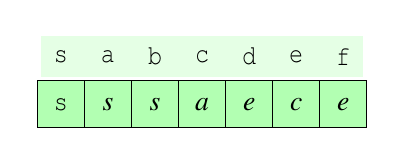
\begin{tikzpicture}[font=\ttfamily,
array/.style={matrix of nodes,nodes={draw, minimum size=7mm, minimum
    width=1.7em,minimum height=1.7em, anchor=center, fill=green!30},column sep=-\pgflinewidth, row sep=0.5mm, nodes in empty cells,
row 1/.style={nodes={draw=none, fill=none, minimum size=5mm}}}]
\matrix[array] (array) {
s & a & b & c & d & e & f\\
s  & $s$ & $s$ & $a$ & $e$ & $c$ & $e$\\};
\begin{scope}[on background layer]
\fill[green!10] (array-1-1.north west) rectangle (array-1-7.south east);
\end{scope}
\end{tikzpicture}
\raisebox{1.3em}{
\begin{tikzpicture}[font=\ttfamily]
\qquad $\;\;\;\;\;d\;\;-\;\;$\quad $distance(s,f)=19$
\end{tikzpicture}}

\textit{Iteration 7}\newline
Delete d from $PQ$ and $S=\{s,a,b,c,e,f,d\}$\newline
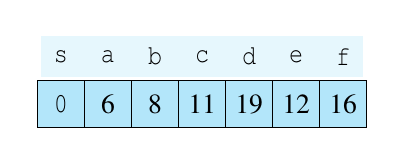
\begin{tikzpicture}[font=\ttfamily,
array/.style={matrix of nodes,nodes={draw, minimum size=7mm, minimum
    width=1.7em,minimum height=1.7em, anchor=center, fill=cyan!30},column sep=-\pgflinewidth, row sep=0.5mm, nodes in empty cells,
row 1/.style={nodes={draw=none, fill=none, minimum size=5mm}}}]
\matrix[array] (array) {
s & a & b & c & d & e & f\\
0  & $6$ & $8$ & $11$ & $19$ & $12$ & $16$\\};
\begin{scope}[on background layer]
\fill[cyan!10] (array-1-1.north west) rectangle (array-1-7.south east);
\end{scope}
\end{tikzpicture}
\qquad
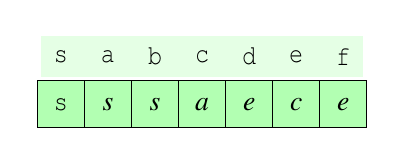
\begin{tikzpicture}[font=\ttfamily,
array/.style={matrix of nodes,nodes={draw, minimum size=7mm, minimum
    width=1.7em,minimum height=1.7em, anchor=center, fill=green!30},column sep=-\pgflinewidth, row sep=0.5mm, nodes in empty cells,
row 1/.style={nodes={draw=none, fill=none, minimum size=5mm}}}]
\matrix[array] (array) {
s & a & b & c & d & e & f\\
s  & $s$ & $s$ & $a$ & $e$ & $c$ & $e$\\};
\begin{scope}[on background layer]
\fill[green!10] (array-1-1.north west) rectangle (array-1-7.south east);
\end{scope}
\end{tikzpicture}
\raisebox{1.3em}{
\begin{tikzpicture}[font=\ttfamily]
\qquad $\;\;\;\;\;\;\;\;\;\;\;\;\;\;\;\;\;\;\;\;\;\;\;\;\;\phi\;$\quad
\end{tikzpicture}}

2. Hence we obtain $prev=[s,s,s,a,e,c,e]$ which yields the shortest-path tree for the graph as depicted in Figure 1.
\begin{figure}[H]
\centering
    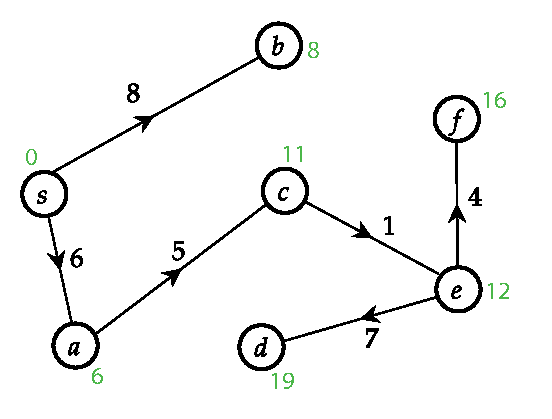
\includegraphics[scale=1.3]{WA3/images/graph1.pdf}
    \caption{Shortest-path tree of the given graph.}
\end{figure}

\newproblem

1. Observe that the given graph $G$ does not have a negative cycle but there is, indeed, a cycle of length zero, namely $c\to d\to e\to c$. We maintain the dynamic programming table $dist(k,v)$ and another table to store the corresponding $pre(k,v)$ values for $v\in V$ and $0\leq k\leq |V|-1=5$. The resulting dynamic programming tables are given below in Table 1 and Table 2. Note that we get $dist=[0,4,7,15,8,1]$ and $prev=[s,s,e,c,f,b]$.

\begin{table}   
\parbox{.45\linewidth}{
\centering
        \begin{tabular}{c|c|c|c|c|c|c|}
              & s & b & c & d & e & f\\
            \hline 
            0 & 0 & $\infty$ & $\infty$ & $\infty$ & $\infty$ & $\infty$\\
            \hline 
            1 & 0 & 4 & 9 & $\infty$ & $\infty$ & $\infty$\\
            \hline 
            2 & 0 & 4 & 9 & 17 & $\infty$ & 1\\
            \hline 
            3 & 0 & 4 & 9 & 17 & 8 & 1\\
            \hline 
            4 & 0 & 4 & 7 & 17 & 8 & 1\\
            \hline 
            5 & 0 & 4 & 7 & 15 & 8 & 1\\
            \hline 
        \end{tabular}
    \caption{$dist(k, v)$}
}
\hfill      
\parbox{.45\linewidth}{
\centering
        \begin{tabular}{c|c|c|c|c|c|c|}
              & s & b & c & d & e & f\\
            \hline 
            0 & s & $\phi$ & $\phi$ & $\phi$ & $\phi$ & $\phi$\\
            \hline 
            1 & s & s & s & $\phi$ & $\phi$ & $\phi$\\
            \hline 
            2 & s & s & s & c & $\phi$ & b\\
            \hline 
            3 & s & s & s & c & f & b\\
            \hline 
            4 & s & s & e & c & f & b\\
            \hline 
            5 & s & s & e & c & f & b\\
            \hline 
        \end{tabular}
    \caption{$prev(k,v)$}
}
\end{table}

2. The shortest-path tree for the $G$ is portrayed in Figure 2 below.
\begin{figure}[H]
\centering
    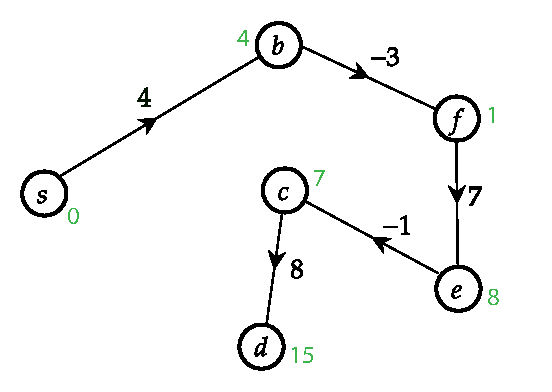
\includegraphics[scale=1.3]{WA3/images/graph2.pdf}
    \caption{Shortest-path tree of $G$.}
\end{figure}

\newproblem
1. Let $l\colon V\to \{0,1,\cdots,9\}$ be the given label map. Observe that if there is a path $s= v_0\to v_1\to\cdots \to v_{n-1}\to v_n=t$ satisfying the 465465... pattern, then 
$l(v_i)= \left\{
\begin{array}{ll}
      4 & if\;i\equiv0\;(mod\;3) \\
      6 & if\;i\equiv1\;(mod\;3) \\
      5 & if\;i\equiv2\;(mod\;3) \\
\end{array} 
\right.$
for all $0\leq i\leq n$. In particular, $l(s)=l(v_0)=4$ for such a path. Moreover, a path satisfying this pattern in $G$ corresponds to a unique path in the digraph $G'=(V',E')$, constructed by letting $V'=V$ and $E'=\{e=(u,v)\in E\mid (l(u),l(v))\in\{(4,6),\,(6,5),\,(5,4)\}\}$, the new path merely being the exact same path projected onto $G'$. Ergo, we first construct $G'$ and then verify that $l(s)=4$ and $t$ is reachable from $s$ in this new graph. Note that this condition is sufficient because if we find a path from $s$ to $t$ in $G'$ satisfying $l(s)=4$, then the inclusion map from $G'\to G$ gives us the required path in $G$ satisfying the 465465... pattern by construction of $G'$. 

\begin{minipage}{0.8\textwidth}
	\aaA {10}{Algorithm PATH-465~($G=(V,E),\,l(v)\;(\forall v\in V),\,s,t\in V$)}\xxx
	\aab {if $l(s)\neq 4$: return false;}\xxx
	\aab {init $G'=(V',E')$ with $V'=V$ and $E'=\phi$;}\xxx
	\aaB {2}{for each edge $(u, v)\in E$}\xxx
	\aac {if $(l(u),l(v))\in\{(4,6),\,(6,5),\,(5,4)\}\}$: add $(u,v)$ to $E'$;}\xxx
	\aab {end for;}\xxx
	\aab {init $visited[\;] = [0] \ast |V|$}\xxx
	\aab {explore$(G',s)$;}\xxx
	\aab {if $visited[\,t\,]=1$: return true;}\xxx
	\aab {return false;}\xxx
	\aaa {end algorithm;}\xxx
\end{minipage}

\textbf{Running time:} Construction of $G'$ takes $O(|V|+|E|)$ time because $V'=V$ and forming $E'$ requires iterating through all edges in $E$. Moreover, explore$(G',s)$ runs in $O(|V'|+|E'|)=O(|V|+|E|)$ time as $|E'|\leq |E|$. Thus, the running time of the algorithm is $O(|V|+|E|)$.

2. The crux of this problem is to perform a breadth first search on $G$ while examining all walks originating from $s$ that follow the 465465... pattern along the edges, until either we find a walk that passes through $t$ or we run out of possible paths. The only issue arises when there is a $3n$-cycle in G of the form $a\to b\to c\to\cdots\to c'\to a$ with $\ell (a,b)=4,\,\ell (b,c)=6,\,\cdots,\,\ell (c',a)=5$ (for example, $c=c'$ when $n=1$) which is reachable from $s$ and there does not exist a walk from $s$ to $t$ satisfying the 465465... pattern. In this case, we need to prevent our algorithm from getting stuck iterating in this cycle. This can be done by making the remarkable observation that if a walk from $s$ to $t$ follows the 465465... pattern, then although it may contain repeated vertices, it cannot contain repeated edges. This is because if an edge $e$ occurs twice in such a walk, say at $v_i$ and at $v_j$, then the subwalk $v_{i+1}\to\cdots\to v_j$ between those two occurrences can be omitted and we will still maintain the 465465... pattern. Hence, all we need to do is keep track of the traversed edges and prevent our algorithm from traversing over them again. Note that we use the formula for $l(v_i)$ given in part 1 to check if our walk satisfies the required pattern and we store vertices $v$ in the queue for BFS along with the label of the edge $(u,v)$, while examining which we had inserted $v$ into the queue. By finding the 'junction' in the queue where the value of these labels changes to the next term in the sequence 465465..., we can know when to proceed to the next level of the graph and thereby the expected label of the following vertex.   

\textbf{Running time:} Since the algorithm below is a modified version of BFS, with the modifications running in constant time, and as every edge is traversed exactly once due to the $traversed[\;]$ array, its running time is $O(|V|+|E|)$.

\begin{minipage}{0.8\textwidth}
	\aaA {24.5}{Algorithm WALK-465~($G=(V,E),\,l(e)\;(\forall e\in E),\,s,t\in V$)}\xxx
	\aab {init $pattern[0\cdots2]=\{4,6,5\};$}\xxx
	\aab {init $level=0$;}\xxx
	\aab {init $traversed[\;]= [0] \ast |E|$;}\xxx
	\aab {init an empty queue $Q$;}\xxx
	\aab {insert$(Q,\,[s,0])$;}\xxx
	\aaB {16.5}{while empty$(Q)=false$}\xxx
	\aac {$a=\,$find-earliest($Q$);}\xxx
	\aac {delete-earliest($Q$);}\xxx
	\aac {init $u=a[0]$; //earliest vertex}\xxx
	\aac {init $label=a[1]$; //label of edge associated with vertex $u$}\xxx
	\aaC {6.8}{for each edge $(u,v)\in E$}\xxx
	\aad {if $traversed[(u,v)]=1$: continue;}\xxx
	\aaD {2.8}{if $l(u,v)=pattern[level\;(mod\;3)]$}\xxx
	\aae {if $v=t$: return true;}\xxx
	\aae {insert$(Q,\,[v,\,l(u,v)])$}\xxx
	\aad {end if;}\xxx
	\aad {$traversed[(u,v)]=1$;}\xxx
	\aac {end for;}\xxx
	\aaC {2.8}{if empty$(Q)=false$}\xxx
	\aad {init $b=\,$find-earliest($Q$);}\xxx
	\aad {if $label\neq b[1]$: level++}\xxx
	\aac {end if;}\xxx
	\aab {end while;}\xxx
	\aab {return false;}\xxx
	\aaa {end algorithm;}\xxx
\end{minipage}

\textbf{Note:} Alternatively, we can attempt this problem by constructing the line graph (also called the conjugate graph) $G'$ of $G$ by interchanging the roles of edges and vertices. More precisely, ${G'=(V',E')}$, where $V'=E$ and $E'=\{(e,e')\mid e=(u,v)$ and $e'=(v,w)$ for some $(u,v),(v,w)\in E$ that share a common vertex $v\in V\}$. Then, by the construction of $G'$, a walk $W:s=v_0\to v_1\to\cdots\to v_n=t$ from $s$ to $t$, where the $v_i$'s are not necessarily distinct, exists in $G$ if and only if there is a path $P:(s,v_1)\to(v_1,v_2)\to\cdots\to(v_{n-1},t)$ in $G'$. Also, such a path $P$ is well-defined because although the vertices in $W$ may repeat, we can suppose that the edges in $W$ are distinct because otherwise we can omit the subwalk between two consecutive occurrences of the same edge. Lastly, $W$ will follow the 465465... pattern along its edges in $G$ if and only if $P$ follows the 465465... pattern along its vertices in $G'$, thereby reducing this problem to calling the algorithm PATH-465$(G'=(V',E'),\,l(e)\;(\forall e\in E),\,(s, x),(y,t)\in E)$ for all possible out-edges $(s,x)\in E$ with $l(s,x)=4$ and in-edges $(y,t)\in E$. Although this algorithm works, its running time is not $O(|V|+|E|)$. Constructing $V'$ takes $O(|E|)$ time. For constructing $E'$, we iterate over all the edges $(u,v)\in E$ and for each edge, we examine the array corresponding to $v$ in the adjacency list and add all edges of the form $((u,v),(v,w))$ to $E'$ for every $(v,w)$ present in $E$. This will take $O(|E|^2)$ if for each edge $(u,v)$, we iterate over all the edges and select the out-edges from $v$. This suggests that the construction of $G'$ should be done in $O(|E|^2)$ time. Moreover, if we look at the worst case scenario of an $n-$clique (with directed edges both ways between any two vertices), then we have $|V|=n$ and so $|E| = {n \choose 2}\cdot 2! = n(n-1)$; thus, by looking at all the possible permutations of $((u,v),(v,w))$, where $u$ and $w$ can repeat, we will have $n(n-1)^2$ edges in $E'$. Adding each such edge to $E$' takes constant time and so adding all of them will take at least $O(n(n-1)^2)=O(n^3)$ time regardless of how we add them to $E'$. But $O(|E|^2) = O(n^4)$ and $O(|V|+|E|) = O(n^2)$. This suggests that an algorithm more efficient than $O(|E|^2)$ might exist but a $O(|V|+|E|)$ time algorithm is likely not possible.

\newproblem
Recall that the optimal substructure property of directed graphs holds for graphs with possibly negative edge lengths. Let $a\in V$ be fixed and $u,v\in V$ be arbitrary. Then by the optimal substructure property, if $P\colon u\to\cdots\to a\to \cdots \to v$ is the shortest path from $u$ to $v$ passing through $a$, then $u \to \cdots\to a$ and $a \to \cdots\to v$ must be the shortest paths from $u$ to $a$ and from $a$ to $v$ respectively, because if there were a shorter path from $u$ to $a$ or from $a$ to $v$, then by replacing this new subpath in $P$, we would obtain a path from $u$ to $v$ passing through $a$ that is shorter than $P$, which is absurd. Hence, $distance_a(u,v)=distance(u,a)+distance(a,v)$, where $distance(x,y)$ is the length of the shortest path from $x$ to $y$. We first call DP-shortest-path$(G,\,l(e)\;(\forall e\in E),\; a\in V)$ which yields the shortest distance $distance(a,v)$ from $a$ to $v$ for all $v\in V$. 
Recall that the DPS-shortest-path algorithm runs in $O(|V|\cdot |E|)$ time. 
Next, we compute $G_R$, the reverse of graph $G$ which takes $O(|V|+|E|)$ time. Note that if $(x,y)\in E$, then $(y,x)\in E_R$ and $l(x,y)=l_R(y,x)$. Hence, $u\to v_1\to\cdots \to v_{n-1}\to a$ is the shortest path from $u$ to $a$ in $G$ if and only if $a\to v_{n-1}\to\cdots\to v_1\to u$ is the shortest path from $a$ to $u$ in $G_R$ because given any path $P=(e_1,e_2,\cdots,e_m)$ in $G$, the corresponding path in $G_R$ is uniquely given by $P_R=(e_m',\cdots,e_2',e_1')$ (where $e=(a,b)\in E\iff e'=(b,a)\in E_R$) and so the lengths of the two paths are the same because $$\sum_{e_i\in P}l(e_i)=l(e_1)+l(e_2)+\cdots+l(e_m)=l_R(e_m')+\cdots+l_R(e_2')+l_R(e_1')=\sum_{e_i'\in P_R} l_R(e_i')$$ Therefore, $distance(u,a)=distance(a,u)|_{G_R}$ for all $u\in V$. Thus, we now call the algorithm DP-shortest-path$(G_R,\,l(e')\;(\forall e'\in E_R),\; a\in V_R)$ which yields $distance(a,u)|_{G_R}$ for all $u\in V$, which in turn gives us $distance(u, a)$ for all $u\in V$, again in $O(|V_R|\cdot |E_R|)=O(|V|\cdot |E|)$ time since $|V|=|V_R|$ and $|E|=|E_R|$. Lastly, we iterate through all the $|V|^2$ pairs $(u,v)$ (note that $u$ and $v$ can be possibly equal and one of them can be possibly equal to $a$) and compute  $distance_a(u,v)$ as $distance(u,a)+distance(a,v)$. This takes $O(|V|^2)$ time. Subsequently, the time complexity of this algorithm is $O(2\cdot|V|\cdot|E|+|V|+|E|+|V|^2)=O(|V|\cdot(|V|+|E|))$ as $|V|,|E|<<|V|^2,|V|\cdot |E|$.

\newproblem
The main idea of this problem is to regard the weight of every vertex as an extension of the lengths of each of its in-edges. To be explicit, given an edge $(u,v)\in E$, the idea is to replace $l(u,v)$ in Dijkstra's algorithm with $l(u,v)+w(v)$. Note that both $l(e)$ and $w(v)$ are positive; thus, $l(e)+w(v)$ is positive and so the invariant of having $distance(s,v)=dist[v]$ once we set $dist[v]$ to a finite value is maintained. Also note that $dist[s]=0+w(s)=0$. Another way to view this problem is to split every weighted vertex $v$ into unweighted vertices $v'$ and $v''$, and add an edge $(v',v'')$ to $E$ with $l(v',v'')=w(v)$, such that all in-edges of $v$ connect to $v'$ and all out-edges of $v$ emerge from $v''$. Then the problem is reduced to running the usual Dijkstra's algorithm on this new graph. Since the length of a path in this modified graph without weighted vertices is equal to the length of the corresponding path in $G$ defined as the sum of lengths of all edges and weights of all vertices in the path, it is clear that this alternate way is essentially equivalent to implementing Dijkstra's algorithm with the weight of each vertex considered as an extension of the lengths of each of its in-edges. The following pseudo-code illustrates the slight modification made to Dijkstra's algorithm.

\definecolor{darkgreen}{rgb}{0.07,0.49,0.06}
\begin{minipage}{0.8\textwidth}
	\aaA {16}{Algorithm Dijkstra-Mod~($G=(V,E),\,l(e)\;(\forall e\in E),\,w(v)\;(\forall v\in V),\,s\in V$)}\xxx
	\aab {$dist[v]=\infty$, for any $v\in V$}\xxx
	\aab {init an empty priority queue $PQ$;}\xxx
	\aab {for each $v\in V$: insert$(PQ,v)$, where the priority of $v$ is $\infty$;}\xxx
	\aab {$dist[s]=0$;}\xxx
	\aab {decrease-key($PQ,s,0$);}\xxx
	\aaB {9.5}{while empty$(PQ)=false$}\xxx
	\aac {$u=\,$find-min$(PQ)$}\xxx
	\aac {delete-min$(PQ)$}\xxx
	\aaC {5.5}{for each edge $(u,v)\in E$}\xxx
	\aaD {3.5}{\color{darkgreen}if $dist[v]>dist[u]+l(u,v)+w(v)$}\xxx
	\aae {\color{darkgreen}$dist[v]=dist[u]+l(u,v)+w(v)$;}\xxx
	\aae {decrease-key$(PQ,v,dist[v])$;}\xxx
	\aad {end if;}\xxx
	\aac {end for;}\xxx
	\aab {end while;}\xxx
	\aaa {end algorithm;}\xxx
\end{minipage}

\textbf{Running time:} Running time of the algorithm is the same as Dijkstra's algorithm since the number of iterations made remains unchanged. So Dijkstra-Mod runs in $O((|V|+|E|)\cdot log|V|)$ time.

\newproblem
In the dynamic programming algorithm for the shortest path problem, observe that when $dist(k,v)>dist(k-1,u)+l(u,v)$, we update $dist(k,v)$ to reflect the current shortest path(s) from $s$ to $v$ using at most $k$ edges; thus, there will be two or more shortest paths from $s$ to $v$ if and only if there are two or more shortest paths from $s$ to $u$, or equivalently if $multiple[u]=1$ (this is because we can traverse from $u$ to $v$ only along the edge $(u,v)$ and so the possibility of multiple shortest paths depends on the scenario between $s$ and $u$). Hence, we need to set $multiple[v]$ to $multiple[u]$, should $dist(k,v)$ be updated. Moreover, if $dist(k,v)=dist(k-1,u)+l(u,v)$ and $prev[v]\neq u$, then we have found at least two distinct shortest paths from $s$ to $v$, one (class of paths) being the current path(s) $s\to\cdots\to prev[v]\to v$ associated with the previous update of $dist(k,v)$ and another (class) being the join of the shortest path(s) from $s$ to $u$ and the edge $(u,v)$. By checking that $prev[v]\neq u$, we ensure that we do not count the current shortest path twice. But then this raises the query about what happens when there are multiple shortest paths of the form  $s\to\cdots\to u\to v$. This is dealt with in the previous case wherein we set $multiple[v]=multiple[u]$ while updating $dist(k,v)$, so all the shortest paths from $s$ to $u$ carry over to the scenario between $s$ and $v$. This exhausts all possibilities for shortest paths from $s$ to $v$. Lastly, our choice of setting $multiple[v]=0$ for all $v\in V$ at the beginning of the algorithm below is justified because all vertices $v\in V$ are reachable from $s$ and so either $multiple[v]=0$ (unique shortest path) or $multiple[v]=1$ (multiple shortest paths). Ergo, the state of the binary array $multiple$ at the end of the algorithm is as desired.

\begin{minipage}{0.8\textwidth}
	\aaA {20.5}{Algorithm DP-multi-shortest-path~($G=(V,E),\,l(e)\;(\forall e\in E),\,s\in V$)}\xxx
	\aab {init a 2D array $dist$ of size $|V|\times |V|$;}\xxx
	\aab {$dist[0,s]=0$;}\xxx
	\aab {$dist[0,v]=\infty$, for all $v\in V\setminus\{s\}$;}\xxx
	\aab {$prev[v]=null$, for all $v\in V$;}\xxx
	\aab {$multiple[v]=0$, for all $v\in V$;}\xxx
	\aaB {12.5}{for $k=1$ to $|V|-1$}\xxx
	\aaC {11}{for $v\in V$}\xxx
	\aad {$dist(k,v)=dist(k-1,v)$;}\xxx
	\aaD {8}{for each edge $(u,v)\in E$}\xxx
	\aaE {2}{if $dist(k,v)=dist(k-1,u)+l(u,v)$ and $prev[v]\neq u$}\xxx
	\aaf {$multiple[v]=1$;}\xxx
	\aaE {4}{else if $dist(k,v)>dist(k-1,u)+l(u,v)$}\xxx
	\aaf {$dist(k,v)=dist(k-1,u)+l(u,v)$;}\xxx
	\aaf {$prev[v]=u$;}\xxx
	\aaf {$multiple[v]=multiple[u]$;}\xxx
	\aae {end if;}\xxx
	\aad {end for;}\xxx
	\aac {end for;}\xxx
	\aab {end for;}\xxx
	\aab {$dist[|V|-1,v]$ gives $distance(s,v)$, for each $v\in V$;}\xxx
	\aaa {end algorithm;}\xxx
\end{minipage}

\textbf{Running time:} Since we have only made slight modifications to the DP-shortest-path algorithm, and these modifications run in constant time, so the running time of the algorithm is the same as the dynamic programming algorithm for shortest path, namely $O(|V|\cdot|E|)$.

\newproblem
Suppose that $P=(e_1,e_2,\cdots,e_n)$ is a path in $G$ with edges $e_i\in E$. Then the probability that $P$ will not fail (reliability) is given by $Pr(P):=\prod_{1\leq i\leq n} r(e_i)$ because all the given probabilities are independent. We want to find the most reliable path from $s$ to $t$, namely the path $P$ from $s$ to $t$ for which $Pr(P)$ is maximum. 
However, Dijkstra's algorithm can only work with graphs wherein the lengths of paths are computed additively and the lengths of all edges are positive. 
Now, observe that maximizing $Pr(P)=\prod_{1\leq i\leq n} r(e_i)$ is equivalent to maximizing $$ln(Pr(P)):=ln\left(\prod_{1\leq i\leq n} r(e_i)\right)=\sum_{i=1}^n ln(r(e_i))$$ because the natural logarithm $ln(\cdot)\colon (0,\infty)\to\RR$ is an increasing monotonic function. 
Now, for every $e\in E$, we have $r(e)\in(0,1)\implies ln(r(e))\in (-\infty, 0)\implies -ln(r(e))\in (0, \infty)$. 
Moreover, maximizing $\sum_{i=1}^n ln(r(e_i))$ is equivalent to minimizing $\sum_{i=1}^n -ln(r(e_i))$. Now, we define a map $\ell\colon E\to (0,\infty)\colon (u,v)\mapsto -ln(r(u,v))$ and $\ell$ is well-defined because given any $e\in E$, $-ln(r(e))\in(0,\infty)$. Ergo, we can now call Dijkstra$(G,\,\ell(e)\;(\forall e\in E),\; s\in V)$ because all the new edge lengths $\ell(e)$ are positive and the length of a path $P=(e_1,e_2,\cdots,e_n)$ in $G$ is computed additively as $\sum_{1\leq i\leq n} \ell(e_i)$. 
This yields the shortest distances from $s$ to all vertices in $V$ and the $pre[\;]$ array, which tells us the path $\gamma:s=v_0\to v_1\to\cdots\to v_{n-1}\to v_n=t$ with the minimum length $\sum_{0\leq i\leq n-1} \ell(v_i,v_{i+1})=\sum_{0\leq i\leq n-1} -ln(r(v_i,v_{i+1}))$, and since this corresponds to the maximum value of the product $\prod_{0\leq i\leq n-1} r(v_i,v_{i+1})$, we conclude that $\gamma$ is the most reliable path from $s$ to $t$.

\textbf{Running time:} Constructing the map $\ell$ takes $O(|E|)$ time and so the running time of Dijkstra's algorithm dominates in the algorithm. Hence, the time complexity of the algorithm is the same as Dijkstra's algorithm, that is $O((|V|+|E|)\cdot log|V|)$.
\end{document}
